\section{Imágenes}

Para usar imágenes dentro del documento, debemos tener en el mismo el paquete \textbf{graphicx} y las imágenes en el directorio del proyecto.

Para adjuntar la imagen o imágenes a un documento se usa el comando siguiente:

\textbf{\textbackslash{includegraphics[]\{\}}}

El primer parámetro entre corchetes contiene el tamaño de la imagen y el segundo parámetro la imagen como tal; hay varias formas de indicar el tamaño, como lo puede ser la escala de la imagen, por medio del comando \textbf{width} (anchura) o \textbf{height} (altura):
\begin{lstlisting}
    \usepackage{graphicx}	% Paquete para usar imágenes y figuras.
    
    \begin{document}
        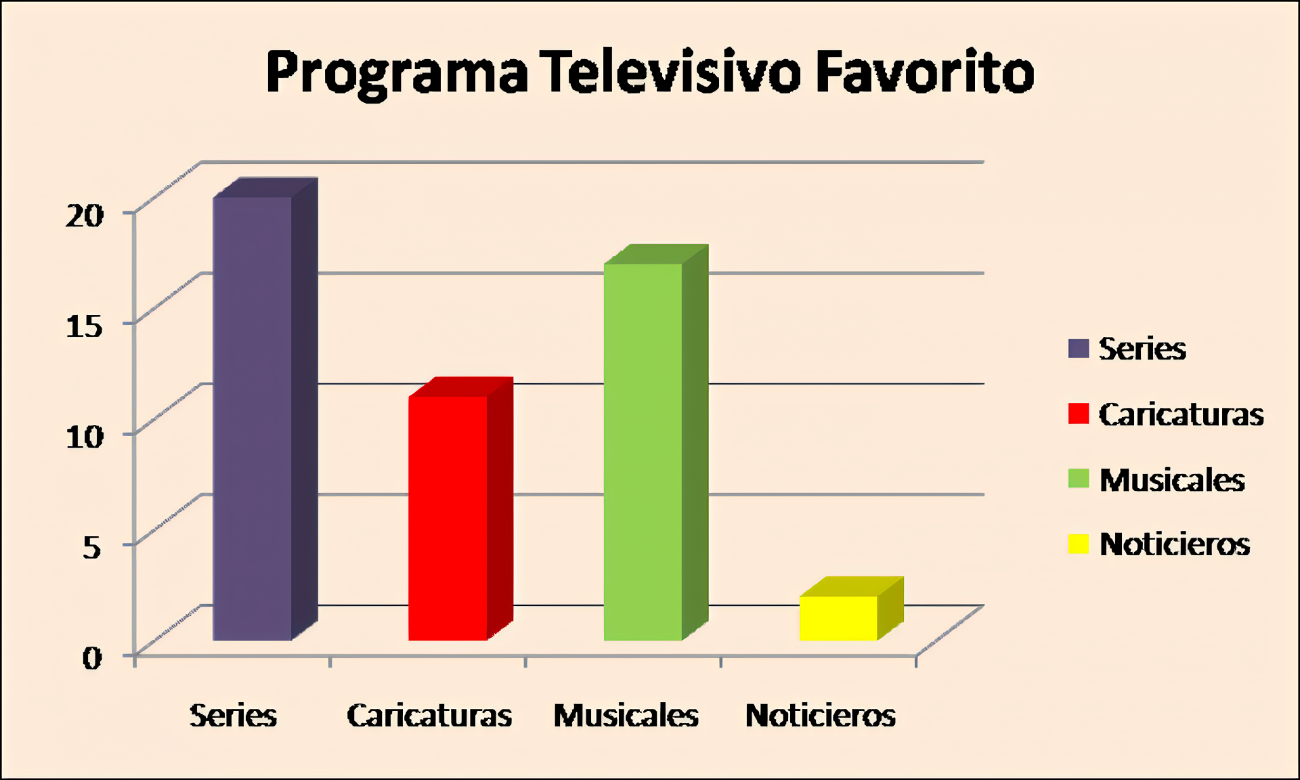
\includegraphics[width=10cm]{ejemplo_latex.png}
    \end{document}
\end{lstlisting}
\begin{figure}[H]
    \begin{center}
    \caption{Imagen de ejemplo}
    \label{fig: 1}
    
\includegraphics[width=10cm]{recursos/logo tecnm.png}
\end{center}
\end{figure}

La \textit{Figura \ref{fig: 1}} posee la dimensión del ejemplo que se acaba de mostrar. Se recomienda trabajar imágenes de forma centrada usando los comando \textbf{\textbackslash{begin\{center\}}} y \textbf{\textbackslash{end\{center\}}} para manejar mejor el comando de inserción de la imagen, su nombre (\textit{caption}) y etiqueta de referencia (\textit{label}).



\section{Listas y secciones}


\subsection{Listas enumeradas}

Para crear una lista numerada, se usa el comando \textbf{\textbackslash{begin}} y \textbf{\textbackslash{end}}, seguido de las llaves donde su contenido es \textbf{enumerate}, con esto se crea una lista numerada, para cada elemento de esta lista se usa el comando \textbf{\textbackslash{item}}:
\begin{lstlisting}
    \begin{enumerate}
        \item LE1
        \item LE2
        \item LE3
    \end{enumerate}
\end{lstlisting}
\begin{enumerate}
    \item LE1
    \item LE2
    \item LE3
\end{enumerate}


\subsection{Listas no numeradas}

Si no se busca una lista numerada, solo se cambia el contenido dentro de las llaves del comando \textbf{begin}, por ejemplo: \textbf{itemize}
\begin{lstlisting}
    \begin{itemize}
        \item LI1
        \item LI2
        \item LI3
    \end{enumerate}
\end{lstlisting}
\begin{itemize}
    \item LI1
    \item LI2
    \item LI3
\end{itemize}

Para hacer listas dentro de listas, basta con comenzar una nueva lista en uno de los items o debajo del comando item.


\subsection{Secciones sin numerar}

Si se desea que los títulos de secciones o subsecciones no estén numerados, se utiliza el ya utilizado comando \textbf{\textbackslash{section}\{\}}, solo que entre el inicio de las llaves y el final de la palabra reservada, se pone un *.
\begin{center}
    \textit{\textbackslash{section*\{Prueba de sección sin enumerar\}}}
\end{center}

\section*{Prueba de sección sin enumerar}



\section{Referencias de un objeto en el texto}

Para referenciar un objeto (tabla, imagen o figura) en \LaTeX se puede usar el comando \textbf{\textbackslash{label\{\}}}, dentro de sus llaves damos nombre al objeto a referenciar. Es importante recalcar que para lograr un referenciado correcto, primero se debe usar el comando \textbf{\textbackslash{caption\{\}}} y después el comando \textit{label}, esto para que no haya errores con el contador de referencias. Además, para llevar un orden en el nombre de las referencias dentro de label, se puede usar la palabra clave \textit{eq}, para ecuaciones; \textit{tab}, para tablas; \textit{img}, para imágenes y \textit{fig}, para figuras.
\begin{lstlisting}
    \caption{Imagen de ejemplo}
    \label{img: 1}
    \caption{Tabla de ejemplo}
    \label{tab: 1}
    \caption{Ecuación de ejemplo}
    \label{eq: 1}
    \caption{Figura de ejemplo}
    \label{fig: 1}
\end{lstlisting}

En este caso, crearé una ecuación con el comando \textbf{\textbackslash{begin}} y \textbf{\textbackslash{end}}, dentro de sus llaves va la palabra \textbf{equation}, el cual numera automáticamente todas las ecuaciones puestas en el documento, y luego la referenciaré en un texto aparte. Para referenciar a las ecuaciones u objetos en otra parte del documento, se usa el comando \textbf{\textbackslash{ref\{\}}}.
\begin{lstlisting}
    \begin{equation}
        \label{ec: 1}
        x^2+2ab+y
    \end{equation}
    
    \begin{equation}
        \label{ec: 2}
        x^2+2ab+y=1
    \end{equation}
    
    La Ecuación \ref{ec: e1} posiblemente está mal escrita. \\
    La Ecuación \ref{ec: e2} igual.
\end{lstlisting}
\begin{equation}
    \label{ec: 1}
    x^2+2ab+y
\end{equation}
\begin{equation}
    \label{ec: 2}
    x^2+2ab+y=1
\end{equation}
La \textit{Ecuación \ref{ec: 1}} posiblemente está mal escrita. \\
La \textit{Ecuación \ref{ec: 2}} igual.
